%%%%%%%%%%%%%%%%%%don't forget if needed %%%%%%%%%%%%%%%%%%%%%
%\section[toc version]{title version%
%              \sectionmark{head version}}
%\sectionmark{head version}
%%%%%%%%%%%%%%%%%%%%%%%%%%%%%%%%%%%%%%%%%%%%%%%%%%%%%%%%%%%%%%
\def\titcourt{Introduction}
\def\titlong{Introduction}
%%%%%%%%%%%%%%%%%%%%%%%%%%%%%%%%%%%%%%%%%%%%%%%%%%%%%%%%%%%%%%%%
\chapter[\titlong]{\titlong%
              \chaptermark{\titcourt}}
\chaptermark{\titcourt}
%%%%%%%%%%%%%%%%%%%%%%%%%%%%%%%%%%%%%%%%%%%%%%%%%%%%%%%%%%%%%%%%
%%%%%%%%%%%%%%%%%%%%%%%%%%%%%%%%%%%%%%%%%%%%%%%%%%%%%%%%%%%%%%%%

Climate change is more than ever experienced in our daily life:
irregular melt of sea, deterioration of ozone layer, non-seasonal precipitation, etc.
Our dependency on fossil fuels during the last decades for energy production have caused severer environmental issues.
%Notwithstanding these alarming phenomenon, those energy sources is still causing severer environmental issues.
%The world's energy consumption was fully dominated by , and 
As shown in Fig. \ref{fig-Energ-cons}a,  coal and natural gas are the main energy sources for electricity generation in the world in 2017 \citep{dudley2018bp}. 
Today, we must face to the fact that these fossil fuels are going to an end and admit that their large utilization has induced considerable impacts on our environment.
%Notwithstanding until today, our dependency on those energy sources is still causing severer environmental issues.
%Climate changing, mostly due to the huge CO2 and other green house gases released into the atmosphere, is more than ever experienced in our daily life:
%unnatural heat waves, non-seasonnal precipitation, seal level rising, increasing melt of sea ice, deterioration of ozone layer, etc.

\begin{figure}[!ht]
\begin{center}
	\begin{minipage}{.49\textwidth}
		(a) \\
		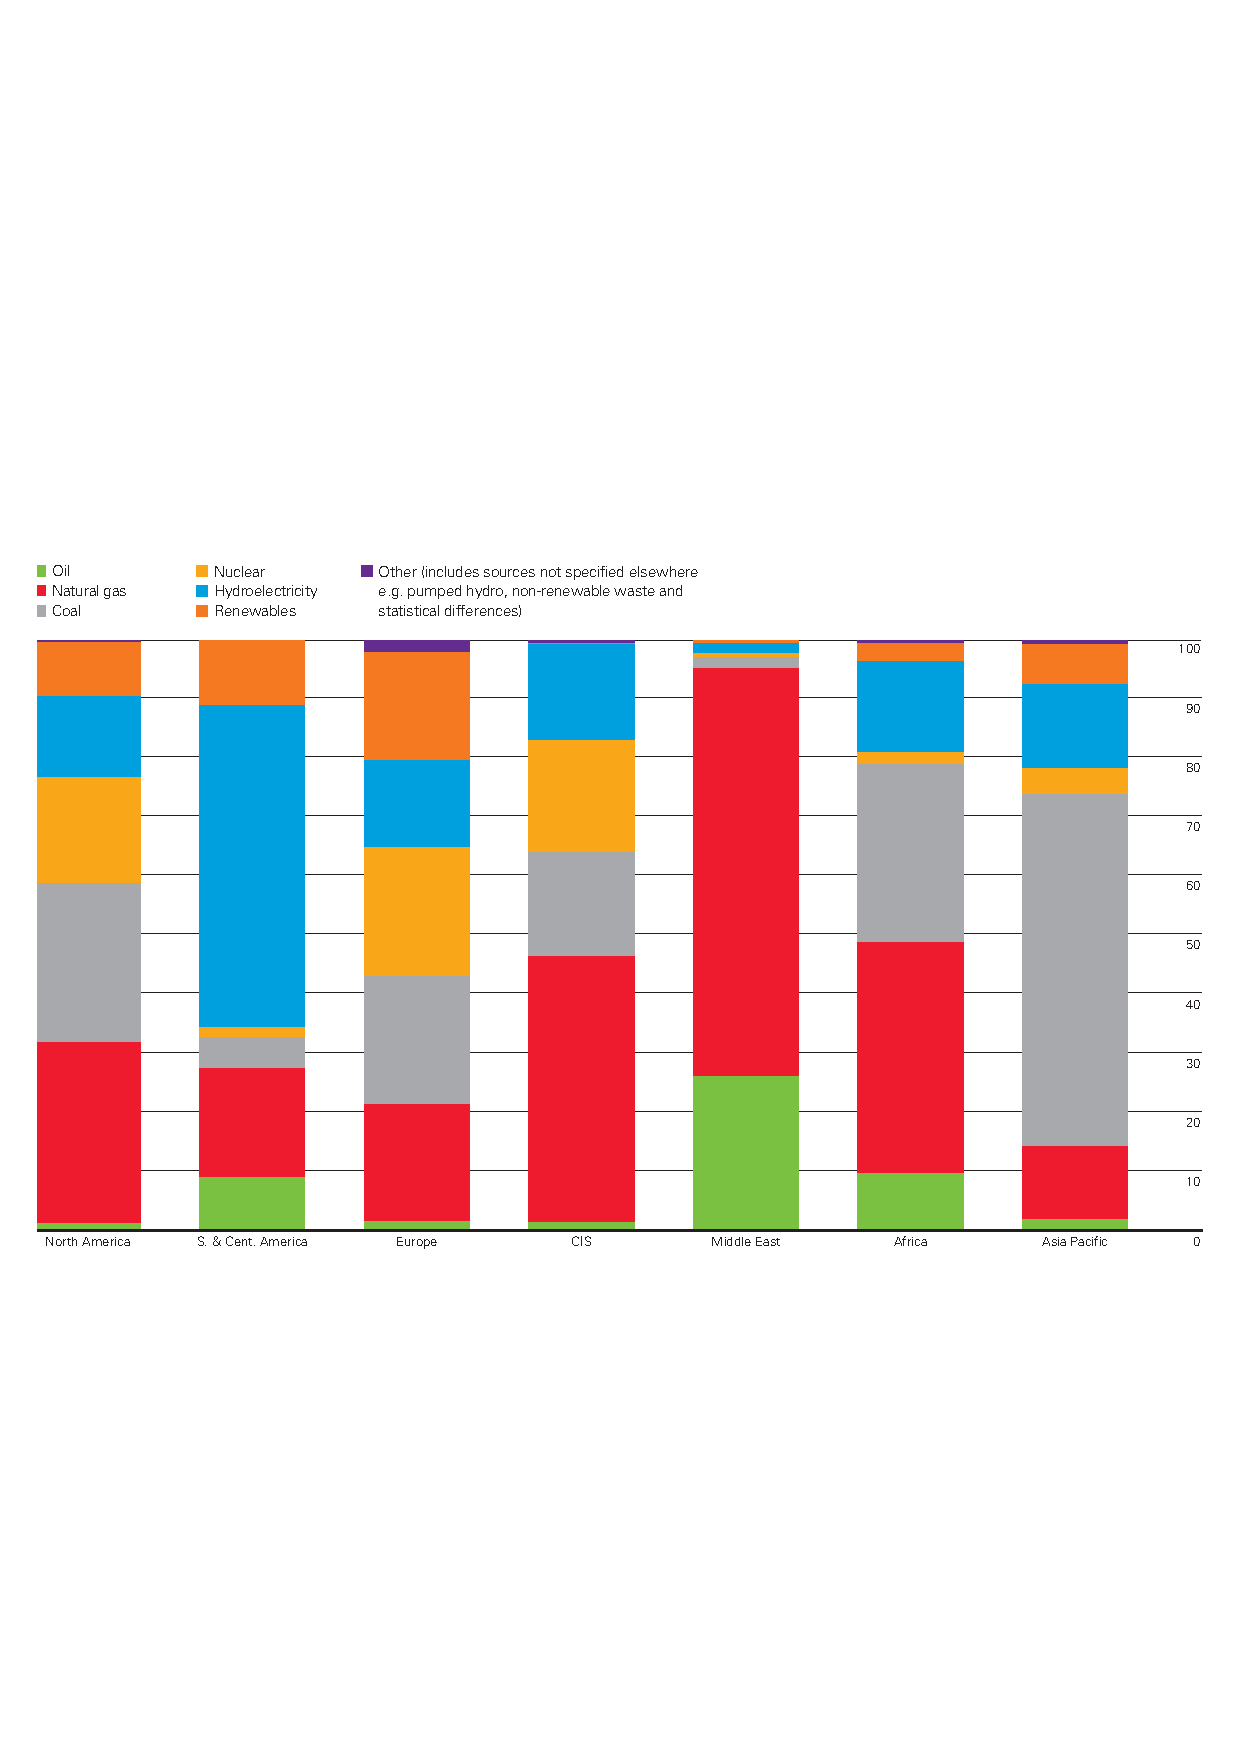
\includegraphics[width=\textwidth]{\figpath/Fig_cap_introduction/Energy_by_continent_2}
	\end{minipage}
		\begin{minipage}{.50\textwidth}
		(b) \\
		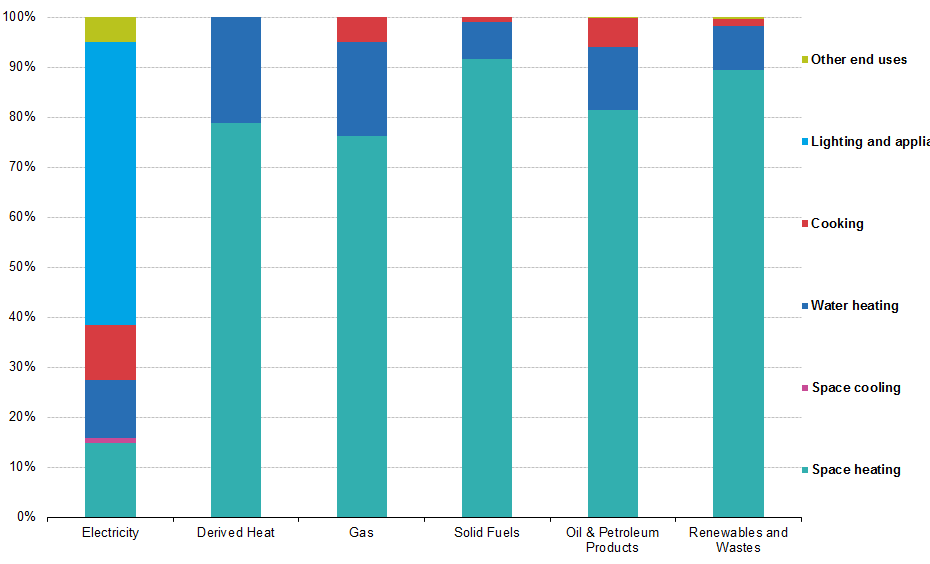
\includegraphics[width=\textwidth]{\figpath/Fig_cap_introduction/Energy-residential-EU}
	\end{minipage}
	\caption{(a) Electricity generation by different energy sources in 2017 by different continent by \cite{dudley2018bp}. (b) Energy use repartition in a residential buildings in Europe by \cite{dudley2018bp}.}
	 \label{fig-Energ-cons}
\end{center}	
\end{figure}

\noindent Research on environment-friendly energy sources, such as biomass, wind or solar have attracted many considerations recently.
Even though solar or wind energy are now operational, their main drawback remains the gap between their availability and the consumers demand.
Solar energy is not available during the nights for example, while wind energy is intermittent over the year.
The energy demand varies with time and the energy suppliers have to meet this demand.

\noindent Current solution to deal with this discrepancies of availability and demands problem is the use of energy storage systems.
The idea is to store the available energy at one time in one form or another and release it latter for a particular need, since energy availability and demand rarely concur.
The energy storage process is a crucial point for renewable and sustainable energy.
The later can be divided into five classes:
magnetic, biological, chemical, mechanical and thermal energy storages.
The main feature of the aforementioned energy storage technologies relies on energy charging and discharging process.
In most cases however, thermal energy is the energy form widely used.
Even the electricity generation is monitored by heat generating high temperature and high pressure.
Storing thermal energy is hence an efficient and fundamental way to store the energy.
It can be realised by rising the substance's temperature (sensible heat energy storage) or by changing the substance's phases (latent heat energy storage).


\begin{table}[!ht]
	\begin{center}
		\begin{tabular}{ccccc}
			Agriculture & Buildings & Industry  & Transportation & Other  \\ \hline
			4.5 & 41.8 & 26 & 43.8 & 4.5 \\
		\end{tabular}
	\end{center}
	\caption {The energy consumed by different domain in France in 2017, in million tonne of oil equivalent. French ministry of ecological transition \citep{ministereEcologie2018}.}
	\label{tab-french-min}
\end{table}

\noindent To this end, research on passive heat storage system have attracted many considerations lastly, namely interest on Phase Change Material (PCM) as a latent heat energy storage have arisen.
PCM are used to store heat during the melting of the materials and releases later the stored energy during the solidification process.
At present, the latent heat storage technologies are proven as an effective solution to decrease the use of fossil fuel and in the same time increase the energy usage efficiency.


Aside from energy storage technologies, PCMs are also widely used in building applications, to decrease the temperature fluctuations.
Latest announcement of the french ministry of ecological transition, detailing the repartition of the energy consumption in different domains, indicates more than $35 \%$ of the total energy being consumed by residentials and commercial buildings. Details about energy consumptions in 2017, reported by the french ministry of ecological transition are shown in Tab. \ref{tab-french-min}.
More than $60\%$ of the total energy consumption in residential sector is dedicated to space heating (see Fig. \ref{fig-Energ-cons}b).
Research towards energy-efficient building to reduce heating and cooling demand is of principal interest nowadays.
Taking advantage of the high value of the latent heat of solid-liquid transformations, PCMs are extensively encountered in buildings thermal regulation to reduce overheating.
In summer, PCMs are used to absorb the excessive solar radiation heat and maintain a bracing indoor ambience.
PCM with a temperature of fusion close to the ambient temperature is generally used to ensure melting during the daytime and solidification during the nighttime.
During winter however, PCMs can be used to store heat generated by electrical heating system during the night and then release it in the daytime.

%The use of efficient insulation is the key of energy conservation in residential buildings.

\begin{table}[!ht]
	\begin{flushleft}
		\begin{tabularx}{\linewidth}{cXX}
					Temperature range & PCM & Target application area \\ \hline \hline
			0 - 65 $^o C$ &    Paraffins (-3 to 64 $^o C$), water / ice  (0 $^o C$), stearic acide  (41 - 43 $^o C$), {n-octadecane  (27.7 $^o C$)}   &   Storage for domestic heating/cooling. Passive storage in bio-climatic building/architecture. Thermal storage of solar energy. Application in off-peak electricity for cooling and heating. Protection of electrical devices.\\ \hline
			%80 - 120 $^o C$ & Erythritol (117.7 $^o C$), RT100  (99 $^o C$),  $MgCl_2 6H_2 O$& \\ \hline
			80 - 120 $^o C$ &    Erythritol (117.7 $^o C$), RT100  (99 $^o C$), $MgCl_2 \, 6H_2O$  (116.7 $^o C$)   &   Storage for the hot-side of $LiBr/H_2O$ absorption cooling system with generator temperature requirements of less than 120 $^o$C\\ \hline
			$ > 150 $ $^o C$ &    $NaNO_3$ (310 $^o C$), $KNO_3$  (330 $^o C$), $NaOH$  (318 $^o C$),  $KOH$  (380 $^o C$), $ZnCl_2$  (280 $^o C$)  &   Storage for solar power plants based on parabolic trough collectors and direct steam generation.\\ 

		\end{tabularx}
	\end{flushleft}
	\caption {Target application area for some PCM studied in the literature \citep{agyenim2010review}.}
	\label{tab-PCM-app}
\end{table}

PCMs are a very timely subject and is encountered in a wide range of applications ranging from metal casting and passive temperature control devices (e.g. for modern portable electronics), to food freezing and cryosurgery.
In many of these applications, the choice of an appropriate material for a specific end depends of many criteria, such as the operating temperature range, the thermal conductivity, the costs, etc.
They are generally classified into three classes: organic, inorganic and eutectic.
A target application area for some PCM is drawn in Tab. \ref{tab-PCM-app}.
The main operating temperature range can be assorted by three groups. First, $0$ to $65 ^o C$ for thermal storage used in domestic heating/cooling or for thermal storage of solar energy. Paraffins and water are used for such applications.
Second, $80$ to $120 ^o C$ for the cooling of systems with generator temperature of less than $120 ^o C$ purpose.
Finally, greater than $150 ^o C$ for the heat storage in solar power plants based on parabolic trough collectors and direct steam generation.
For more details about these applications see \citep{agyenim2010review}.

Melting and solidification are also fundamental process in geophysical problem such as Earth's mantle formations, lava lakes \citep{davaille1993thermal}, thermal convection in magma chambers \citep{brandeis1989convective} or ice-melt lakes \citep{polashenski2012mechanisms}. Ice-melt ponds that form during summer season in the Arctic are known for example to display natural convection coupled to a phase-change process on the bottom side \citep{polashenski2012mechanisms,esfahani2018basal}. 
In that case, Rayleigh-B�nard like convection cells are observed in the liquid phase.

The solid-liquid phase-change phenomenon is known to involve tricky processes. 
It couples the natural convection in the liquid phase induced by the buoyancy force, the non-linear evolution of the phase-change interface and the heat transfer process, which could be different from one configuration to another.
The coupling of all these physical phenomenons induces strong non-linear process in the solid-liquid problems, difficult to analyse except for simple and ideal test cases.
Fig. \ref{fig:expe-PCM_Gong} showing the experimental investigation of the melting of n-octadecane inside a transparent brick, used as a smart material to control the indoor environment of a building by \cite{gong2015numerical}, displays very well the complexity of the problem.
The investigated material is heated from the right and melts consequently from the right to the left.
Figs. \ref{fig:expe-PCM_Gong}a and \ref{fig:expe-PCM_Gong}b indicate the evolution of the liquid fraction and the vector field in the fluid obtained by particle image velocimetry (PIV) method.
Capturing accurately the non-linear evolution of the solid-liquid interface, due to the strong convection in the melting PCM, is clearly a challenging numerical task.
Furthermore, the existence of boundary layers near the walls and the interface suggests that the mesh resolution should allow to capture these structures.

\begin{figure}[!ht]
	\begin{center}
		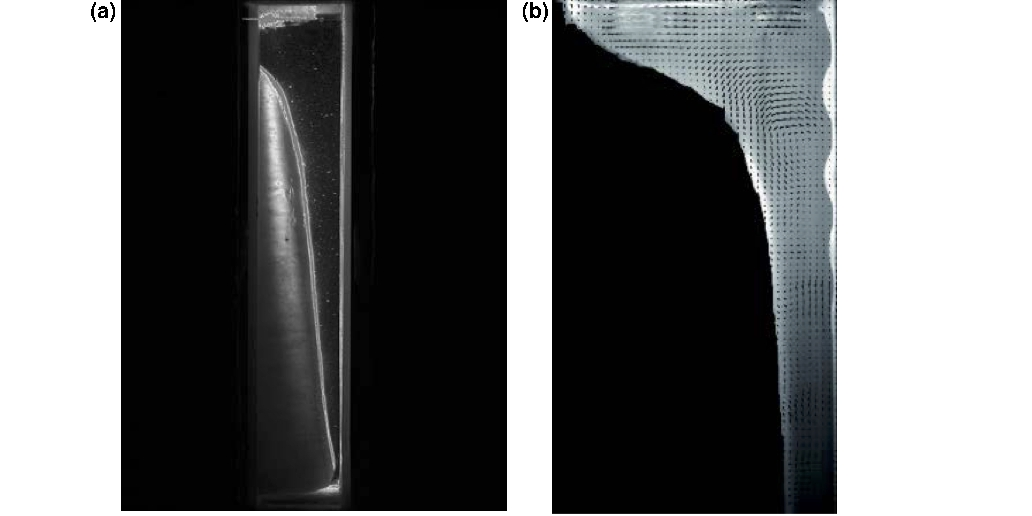
\includegraphics[width=\textwidth]{\figpath/Fig_cap_melting/EXPE_GONG_melting}
	\end{center}
	\caption{Experimental observation of the melting of n-octadecane within a transparent brick of plexiglas heated vertically from the left by \cite{gong2015numerical}, obtained by particle image velocimetry (PIV) method (a) melt fraction (b) velocity field in the liquid region.}
	\label{fig:expe-PCM_Gong}
\end{figure}

Solid-liquid phase-change problem have attracted attention since the study of crust formation of earth by \cite{lame1831memoire}  or the ice formation problem by \cite{stefan1889uber}.
From a mathematical point of view, the phase transition is referred to a moving boundary problem.
The Stefan problem considers a linear evolution of the interface by assuming conductive heat transfer only in the liquid phase.
In the frame of such assumption, the existence and the uniqueness of the solution for the one-dimensional problem was proven by \cite{rubinstein1947solution} using constant properties.
For an historical review detailing the evolution of the Stefan problem and the progressive consideration of convection in the liquid one can refer to \cite{yao1989melting}.
Over the past $30$ years, solid-liquid phase-change involving natural convection has been widely studied. % using either numerical, analytical, or experimental methods.
Rectangular and cylindrical geometries were the most investigated configurations.
\cite{Okada1984,gau1983flow,gong2015numerical} have investigated experimentally the melting of n-octadecane and gallium PCMs inside rectangular containers.
\cite{ho1984inward,liu2014experimental,omojaro2017study} have studied experimentally the melting of different paraffin within cylindrical enclosures.
These experimental investigations have been extensively used for numerical validations (see \cite{bertrand1999melting,gobin2000melting,wang2010numerical,dan-2014-JCP,rakotondrandisa2019numerical}) and have permitted a better comprehension of the physical phenomenon that occurs during melting and solidification, mainly the heat transfer process.
%The experimental results are very often formulated in the form of mathematical correlations.
Experimental work of \cite{Okada1984} have permitted for example to express correlations of the variation of dimensionless thermal energy stored as latent heat. % and the average Nusselt number on the vertical wall with the dimensionless time.
Later, \cite{ho1984inward} have analyzed the solid-liquid interface position for different configuration and \cite{jany1988scaling} have formulated $N\!u$-$\Ray$ correlation through a scaling analysis.
\cite{bejan1989analysis} gathered the previous observations and described analytically the solid-liquid melting process in the frame of vertical heating.
Gallium and n-octadecane were the most investigated materials. 
%Experimentals \citep{gau1983flow,Okada1984,campbell1994visualization,gong2015numerical}, numericals \citep{rady1996natural,bertrand1999melting,hannoun2003resolving,Wang2010,dan-2014-JCP,rakotondrandisa2019numerical}, and theoreticals \citep{Okada1984,jany1988scaling,bejan1989analysis,kowalewski2004phase} works were  performed. 
Besides their physical properties are equal in both liquid and solid phases (differences less than $3 \%$), gallium and n-octadecane melt near room temperature, making them the preferred materials for experimentally investigating melting and solidification of low and high Prandtl-number PCMs respectively.
%These problems in a rectangular cavity have been also extensively used in the literature for the assessment of phase-change numerical methods

The previously mentioned works were mostly focused on studying separately melting or solidification problems
and only recently for alternate melting and solidification complete cycles \citep{wang2010numerical,rakotondrandisa2019numerical}. 
Prior to these studies on complete cycles, periodic melting and solidification problems were the most studied in the literature. 
\cite{ho1993periodic} and \cite{voller1996cyclic} studied numerically, periodic melting in square enclosures. 
Recently, \cite{hosseini2014experimental} carried out melting and solidification of a cylindrical PCM during charging and discharging process and \cite{chabot2017solid} studied analytically the effect of an alternate heating and cooling in a cylindrical PCM, with periodical boundary conditions.
We have also contributed recently on the comprehension of the governing mechanism during the melting and the solidification process in the paper \cite{rakotondrandisa2019numerical}.
We analysed in detail the difference between solidification occuring after a partial melting and a complete melting by providing temporal evolution of solid-liquid interface, liquid fraction, Nusselt number and accumulated heat input. 

While publication about melting and solidification of PCM heated from the side is very abundant, research on melting of PCM heated from below is quite rare.
\cite{diaz1984visualization,hale1980solid} have studied experimentally the solid-liquid interface morphology of PCM during basal heating.
\cite{gong1998flow} studied numerically the flow and heat transfer during the melting of pure n-octadecane in a rectangular cavity heated from below.
Recent numerical simulations have investigated different boundary conditions such as
periodic configurations along the horizontal axis \citep{esfahani2018basal,madruga2018dynamic,favier2019rayleigh} or wavy surface in a rectangular cavity heated from below \citep{kousksou2014melting}.
With regard to theoretical works, \cite{vasil2011dynamic,favier2019rayleigh} have studied the hydrodynamic instabilities at the onset of convection and compared their observation with the classical Rayleigh-B�nard instability mechanism \citep{chandrasekhar2013hydrodynamic}.
\cite{favier2019rayleigh} have focused their attention to the effect of the non-planar topography of the interface to the convection flow.
 On the other hand, \cite{gong1998flow,esfahani2018basal,madruga2018dynamic} mostly focused on global quantities such as the heat flux and the statistical properties of the interface.


\section{Purpose of the thesis}
The purpose of the present work is to investigate numerically solid-liquid phase-change systems.
The investigation tool used in this thesis is the open-source software FreeFem++ \citep{freefem,hecht-2012-JNM}.
A high accuracy numerical model using a Newton method with an adaptive finite element is used to simulate phase-change problems involving natural convection.

\noindent A first investigation on the numerical simulation of convective phase-change problems using adaptive finite element method have been carried out by \cite{dan-2014-JCP}.
The method used consists of solving the Navier-Stokes-Boussinesq equations by the mean of single domain approach using first order scheme.
The technique of variable viscosity approach was applied to annihilate the velocity in the solid phase.
The study was focused on two-dimensional square cavity configuration.

A first objective of this thesis is to improve the existing code, developed by the numerical methods and applications group of the LMRS Laboratory \footnote{http://lmrs-num.math.cnrs.fr}, and to organize the program as a toolbox for the software FreeFem++.
To this end, the objectives are listed as follows: 
\begin{enumerate}[label=(\roman*)]
\item increase the accuracy by using  a second order scheme for the time discretization and $\PP_2$ finite element for the temperature, 
\item implement a Carman-Kozeny model, in addition to the viscosity-based approach, to annihilate the velocity in the solid region, 
\item investigate challenging cases by simulating complex geometries (highly distorted mesh, cylindrical PCM with inner heated tubes) and computationally demanding cases (high Rayleigh numbers), 
\item simulate the complete melting-solidification cycle of a PCM. 
\end{enumerate}
A second objective is to extend the program to three-dimensional configurations.
The two dimensional assumption is indeed no more valid for high Rayleigh problems, especially for basal melting cases.
Moreover, three dimensional adaptive finite element method for convective melting problem is less investigated in the literature.

A third objective is to provide a thorough analysis of both melting and solidification process using the developed tools.

\newpage
\subsection{Existing method for modeling phase-change materials}
%Solid-liquid phase-change problems are encountered in numerous practical applications, ranging from metal casting and thermal energy storage (phase-change materials) to food freezing and cryosurgery. Melting and solidification are also fundamental processes in geophysical problems, such as Earth's mantle formation, lava lakes or magma chambers. 

Temperature gradients induce buoyancy forces in the liquid (melted) phase and generate a significant convective flow.
The appropriate mathematical description of the liquid phase is thus the usual model for the natural convection flow: the incompressible Navier-Stokes system of equations  with Boussinesq approximation for thermal (buoyancy) effects (\eg \cite{viskanta1985natural}). 
In this model, the energy conservation equation is written as a convection-diffusion equation for the temperature. 
In the solid phase, conduction is the main phenomenon and the appropriate model is the classical heat equation. 
The main modelling difficulty is to link these two models by taking into account the separation of the two phases by a sharp interface, across which thermodynamic properties are discontinuous. 

We offer in this section a description of the two main approaches suggested in the literature to deal with solid-liquid phase change problem.  
For a comprehensive review of models for phase-change problems with convection, see \cite{kowalewski2004phase}.  Note that a different category of models was recently suggested in the literature, based on the Lattice Boltzmann Method \citep{luo2015lattice,gong2015numerical} or meshless methods \cite{atluri2002meshless}.  Such methods based on non-deterministic models are not discussed in this introduction.

A first modelling  approach, usually referred to as the multi-domain (or deforming-grid) method, is based on the classical Stefan two-phase model. Solid and liquid domains are separated and the corresponding conservation equations are solved in each domain. Boundary conditions at the interface between domains are obtained by imposing the Stefan condition (balance  of heat fluxes at the interface). The position of the solid-liquid interface  is tracked and moved explicitly using  either {\em front tracking} or  {\em front fixing} methods. The  former method uses deforming grids to reconstruct the interface, while the latter is based on a time-depending coordinate transform, mapping the physical domain into a fixed computational domain. For a detailed description of these methods, see \eg \cite{sparrow1977analysis,unverdi-JCP-1992,gupta2000moving,Tenchev2005}. The main drawback of deforming-grid methods is their algorithmic complexity, which makes difficult to accurately capture solid-liquid interfaces of complicated shape or structure (\eg with mushy regions between solid and liquid phases). Configurations with multiple interacting interfaces (see the solidification of a phase-change material presented in this work) are also difficult to simulate with these methods (see also \cite{kowalewski2004phase-stella}). 

The second modelling approach avoids to impose explicitly the Stefan condition at the solid-liquid interface and therefore uses a single-domain (or fixed-grid) model. The same system of equations is solved in both liquid and solid phases. The energy balance at the interface is implicitly taken into account by the model. Consequently, the position of the interface is obtained a posteriori by post-processing the computed temperature field. Phase-field methods \citep{fabbri-JCP-1997} and enthalpy methods \citep{Voller-1987,Cao1989} are the most commonly used single-domain models. In phase-field methods, a supplementary partial differential equation for the evolution of the order parameter (a continuous variable taking the value 0 in the solid and 1 in the liquid) has to be solved, coupled with the conservation laws \citep{shyy-1996}. This new equation is model dependent and its numerical solution could lead to diffuse solid-liquid interfaces.  For recent contributions in this area, see \cite{boettinger2002phase,singer2008phase,favier2019rayleigh}. We focus below on enthalpy methods, which are the most widely used single-domain models due to their algorithmic simplicity. 

\noindent The main idea behind enthalpy models is to formulate the energy conservation law in terms of enthalpy and temperature and include latent heat effects in the definition of the enthalpy. The obtained equation applies to both liquid and solid phases and implicitly takes into account the separation of the phases. Another advantage of enthalpy methods, when compared to previously described models, is to  remove the limitation of the phase-change occurring at a fixed temperature. The presence of mushy regions can be easily modelled  with these methods. Two types of formulations of enthalpy methods exist in the literature, depending on the main variable used to solve the energy equation: enthalpy or temperature-based methods. \\
In enthalpy-based formulations  the main variable is the enthalpy \citep{eyres1946calculation,rose1960method,bhattacharya2014enthalpy}.  Temperature is computed  from the temperature-enthalpy coupling model. An iterative loop is necessary to solve the energy equation, formulated with both enthalpy and temperature variables. For a review of different iterative techniques to solve the energy equation, see \cite{Voller-1996-chapter}.  A second variety of enthalpy-based formulations consists in rewriting the energy equation with enthalpy terms only \citep{rady1996natural,hannoun2003resolving}. \\
In temperature-based formulations, the energy equation is formulated in terms of temperature only. The latent heat is  treated either by deriving an apparent heat capacity coefficient to define the total enthalpy \citep{Morgan-1978,chiesa1974natural,gau1984melting}  or by introducing a source term in the energy equation \citep{Voller-1996-chapter,swaminathan1997towards}. Advantages and drawbacks of each approach are discussed in detail in \cite{konig2017comprehensive}.

Single-domain methods are very appealing for numerical implementations. The same system of equations is solved in the entire computational domain, making possible algorithmic or computer-architecture optimisations. If enthalpy models offer an elegant solution to deal with the same energy conservation equation in both phases, a last modelling problem has to be solved. It concerns the  extension of the  Navier-Stokes-Boussinesq equations from the  liquid to the solid phase. 
Different techniques to bring the velocity to zero in the solid region were suggested. 

\noindent The most straightforward is the switch-off technique, which decouples solid and liquid computational points and overwrites the value of the velocity by setting it to zero in the solid region. Different implementations of this technique with finite-volume methods are presented in \cite{Ma2006,Wang2010}. 

\noindent In variable viscosity techniques \citep{gartling-1980,voller1987pcm,Cao1990}, the fluid viscosity depends on the temperature and is artificially increased to huge values in the solid regions through a regularisation or mushy zone. To avoid blow-up or numerical inconsistencies, the large gradients of viscosity must be correctly resolved in the mushy region.  
This is naturally achieved in finite-element methods with dynamical mesh adaptivity   \citep{dan-2014-JCP}, while in finite-volume methods with fixed grids, the time step has to be adapted to the space resolution \citep{Ma2006}. Versions of the variable viscosity approach suggested in  \cite{dan-2014-JCP} were further studied by \cite{aldbaissy2018full,WOODFIELD-2019} and implemented in a different finite-element framework (FEniCS) by \cite{zimmerman-2018}.

\noindent A third technique used to ensure a zero velocity field in the solid phase is the so-called enthalpy-porosity model \citep{Brent-1988}.  A penalisation source term is introduced in the momentum equation to allow the switch from the full Navier-Stokes equations in the liquid phase to a Darcy equation for porous media. The mushy region is thus regarded as a very dense porous medium that sharply brings the velocity to zero in the solid region. The expression of the penalisation source term generally follows the Carman-Kozeny model for the permeability of  a porous medium \citep{hannoun2003resolving,hannoun2005,Belhamadia2012}, but other mathematically equivalent expressions were suggested \citep{Angot-1999,favier2019rayleigh}. Different formulations and implementations of the enthalpy-porosity model are presented in \cite{Kowalewski-1999,Giangi-2000,kowalewski2004phase-stella}.

Concerning the space discretization of these models, finite difference (FD) or finite volume (FV) methods are generally used in the literature. 
When single-mesh models are used, the general strategy to capture the solid-liquid interface is to dramatically increase the mesh resolution in the whole domain. 
This results in a considerable increase of the computational time, even for two dimensional cases. 
 \citep{hannoun2003resolving} have reported that the simulation of the melting of tin within $200 \times 200$ fixed grid  required $2,400$ CPU hours, $111$ runs (restarts), and $3$ months of calculations.
Dynamical mesh adaptivity becomes in this context a valuable tool  to concentrate the grid refinement effort only in regions displaying high gradients of the computed variables (melting-solidification fronts, thermal or viscous boundary layers, recirculation zones). 

\noindent Finite  element (FE) methods offer this possibility to dynamically refine the mesh only in specific regions of the domain. %where sharp phenomena takes place (\eg solid-liquid interface, recirculation zones). 
Different FE approaches were suggested, from enthalpy-type methods (\eg \cite{elliott1987error}) to front-tracking methods (\eg \cite{CHLi}). 
Recently, adaptive FE methods were proposed for classical two-phase Stefan problem \citep{Belhamadia2004_S} using an anisotropic mesh adaptation algorithm based on solution-dependent metrics.
The authors extended  their algorithm for the three-dimensional simulation of the same problem  \citep{Belhamadia2004_3D} and showed that the use of locally adapted meshes with strong anisotropy proved to be very effective in reducing the number of computational nodes for such phase-change systems without convection.

\noindent To simulate melting or solidification problems with convection,  \cite{dan-2014-JCP}  recently suggested a dynamical mesh adaptation algorithm based on metrics control and implemented with the \ff software \citep{freefem,hecht-2012-JNM}. 
%and phase-change systems with convection  \citep{Belhamadia2012,dan-2014-JCP}. 
%For the classical two-phase Stefan problem, \cite{Belhamadia2004_S} suggested  an anisotropic mesh adaptation algorithm based on solution-dependent metrics. 
The advantage of this adaptive finite-element method, which will be also used in the present study, is to make possible, with reasonable computational cost, the re-meshing of the computational domain at each time step. 
A very refined discretization of the  regularization zone between solid and liquid phases is thus obtained, while regions with low gradients are de-refined in order to balance the overall computational effort. 

\subsection{Present numerical approach for modeling phase-change materials}
The present work is based on a single-domain enthalpy-porosity model for solid-liquid phase change problems with convection. 
For the energy conservation equation, a temperature-based formulation takes into account the latent heat by introducing  a discontinuous source term. 
For the mass and momentum conservation equations, we solve in the entire domain the incompressible Navier-Stokes equations with Boussinesq approximation for buoyancy effects. 
To bring the velocity to zero in the solid phase, we introduce in the momentum equation a penalty term following the Carman-Kozeny model.  
The coupled system of momentum and energy equations is integrated in time using a second-order Gear scheme. 
All the terms are treated implicitly and the resulting discretized equations are solved using a Newton method \citep{dan-2014-JCP}. 

\noindent The advantage of this formulation is to  permit a straightforward implementation of different types of non-linearities.
For the space discretization we use Taylor-Hood triangular finite elements, \ie $\PP_2$ for the velocity and $\PP_1$ for the pressure. 
Temperature is discretized using $\PP_2$ or $\PP_1$ finite elements. 
Discontinuous variables (latent heat, thermal diffusivity, etc) at the solid-liquid interface are regularized through an intermediate artificial mushy region.

\noindent Single domain methods require a refined mesh near the interface, where large enthalpy gradients have to be correctly resolved. 
An optimized dynamical mesh adaptivity algorithm allows us to adapt the mesh every time step and thus accurately capture the evolution of the interface.  
Mesh adaptivity, feature of the current method, offers the possibility to deal with complicated phase-change cases, involving multiple solid-liquid interfaces.

\noindent There are three main novelties in the present numerical approach, when compared to  \cite{dan-2014-JCP}: 
\begin{enumerate}[label=(\roman*)]
\item we use the Carman-Kozeny model to bring the velocity to zero inside the solid phase, instead of a  viscosity penalty method (imposing a large value of the viscosity in the solid), 
\item we increase  the time accuracy of the algorithm by replacing the first-order Euler scheme with the second-order Gear (BDF2) scheme (see also \cite{Belhamadia2012}), 
\item we improve the metric calculation procedure for mesh adaptivity.
\end{enumerate}

The programs were built and organized as a toolbox for \ff \citep{hecht-2012-JNM,freefem}, which is a free software (under LGPL license). \ff\footnote{\ff for different OS can be downloaded from \texttt{http://www3.freefem.org/}.} offers a large variety of triangular finite elements  (linear and quadratic Lagrangian elements, discontinuous $\PP_1$, Raviart-Thomas elements, etc.)  to solve partial differential equations. It is an integrated product with its own high level programming language and a syntax close to mathematical formulations, making the implementation of numerical algorithms very easy. Among the features making \ff an easy-to-use and highly adaptive  software we recall the advanced automatic mesh generator, mesh adaptation, problem description by its variational formulation, automatic interpolation of data, colour display on line, postscript printouts, etc. The \ff programming framework offers the advantage to hide all technical issues related to the implementation of the finite element method. It becomes then easy to  use the present toolbox to code new numerical algorithms for similar problems with phase-change.

%In this thesis, we use an enthalpy method with a temperature-based formulation using heat source term approach to simulate phase-change systems with convection.
%The natural convection flow in the liquid phase is simulated by solving the full incompressible Navier-Stokes equations with Boussinesq approximation.
%A Carman-Kozeny type penalty model is applied to ensure a zero velocity value in the solid region.
%The main feature of our numerical approach is the use of an adaptive finite element method to accurately track the solid-liquid interface.
%Single domain method requires actually a fine mesh near the phase change front in order to capture the large enthalpy gradient. 
%The smaller the phase change interval the narrower the mushy region and the more refined the mesh should be.
%Yet applying a fine mesh in the whole domain would increase considerably the computational time.
%Hence, we introduce a FE method with time-dependent mesh adaptivity by metric control that is  effective for a large range of phase-change systems with convection, from melting to solidification. The proposed mesh refinement strategy has the capacity to take into account different metrics and thus the ability to refine the mesh in different regions of interest in the computational domain. In particular, we show that the method is able to simultaneously track several interfaces in the domain.\\ 
%The nonlinear system of equations are solved by means of a Newton algorithm.
%A fully-implicit Newton method for the phase-change system based on a finite-element formulation of the Navier-Stokes equations has been derived by \citep{dan-2014-JCP}.
%The advantage of this formulation is to  permit a straightforward implementation of different types of non-linearities in the system of equations.
%
% The code was built as a toolbox for FreeFem++ \citep{hecht-2012-JNM,freefem}, which is a free software (under LGPL license) using a large variety of triangular finite elements  (linear and quadratic Lagrangian elements, discontinuous P$_1$, Raviart-Thomas elements, etc.)  to solve partial differential equations. FreeFem++ is an integrated product with its own high level programming language and a syntax close to mathematical formulations, making the implementation of numerical algorithms very easy. Among the features making FreeFem++ an easy-to-use and highly adaptive  software we recall the advanced automatic mesh generator, mesh adaptation, problem description by its variational formulation, automatic interpolation of data, colour display on line, postscript printouts, etc. FreeFem++ community is continuously growing, with  thousands of users all over the world.

\section{Thesis plan}
Chapter \ref{chap-NSB} sets the mathematical and physical basis of the numerical system used to simulate phase-change problems involving natural convection flow.
We present in detail the incompressible Navier-Stokes-Boussinesq equation and the single-domain approach to solve the same system of equations throughout the whole domain.
The enthalpy method, modeling the phase-change phenomenon is presented first.
The Navier-Stokes equation with Boussinesq approximation to simulate the natural convection in the liquid flow is then developed.
Finally, the final non-dimensional system of equations is described in detail with a discussion about the Carman-Kozeny model used as a penalty term in the momentum equation.

Chapter \ref{chap-FEM} is devoted to the numerical algorithm for solving the numerical system presented previously.
The finite element algorithm we have developed in this work is first presented in detail: time integration scheme, finite element discretization and the Newton method.
The characteristics Galerkin method, an alternative for the treatment of non-linear term in the momentum equation, is also presented.
Then, we describe the mesh adaptivity by metric control, which is a standard function offered by FreeFem++.
Some theoretical tests to assess for the accuracy of our numerical method is also presented.
The space and the time convergence orders are demonstrated using the Burggraf flow and a manufactured solution designed for the incompressible Navier-Stokes equation.
The structure of the new finite-element toolbox for the simulation of PCMs is also described.
The program architecture and the parameter details are presented.
Finally, the domain decomposition method used for large scale simulation is described.

A first validation of our numerical method is addressed in Chapter \ref{chap-NATCONV}.
The capability of the code to deal with linear and non-linear forms of the buoyancy force in the Boussinesq approximation is first tested.
%Differentially heated cavity (horizontal $\nabla T$) configuration is used to compare our results with benchmarks solution existing in the literature.
The test cases are presented by increasing progressively the difficulty.
We simulate first the natural convection of air in square enclosures differentially heated from the vertical walls.
Then heated obstacle is added in the center of the domain.
Finally, we add non-linearity by simulating the natural convection of water.
%Three-dimensional simulations of the natural convection of air is also presented.
%For both two and three-dimensional configurations, qualitative and quantitative validations are provided.

Once the capability of our algorithm to deal with natural convection issues was demonstrated, much more attention to phase-change problem is paid.
Numerical simulation of melting and solidification of PCM is considered in Chapter \ref{chap-MELTING}.
The melting of octadecane and gallium inside rectangular enclosures are investigated first since they were extensively used for numerical method validations, because of their physical properties relatively equal in both solid and liquid phases.
Finally, several PCM container geometries are simulated to prove the robustness of our numerical method, mainly cylindrical and irregular domain are computed.
%Finally, numerical simulation of three-dimensional configuration is presented.

Numerical and scale analysis are investigated in Chapter \ref{chap-MELTING-ANALYSIS}.
We compare the behavior of the PCM when lateral and basal heating are of interest.
The melting of octadecane heated from the side is carried out first.
Then numerical results for the melting from below is performed.
For  both cases, we provide detailed description of the melting process with scaling analysis to better understanding the heat transfer mechanism.
%Accurate comparison is carried out for the differentially heated cavity case, by considering different size of the cavity and different temperature difference between the hot temperature and the temperature of fusion, which are the main parameters monitoring the natural convection in the melting PCM.
Analysis of the time evolution of some physical parameters, such as the Nusselt number, the liquid fraction, the accumulated heat input and the time evolution of the melting are discussed. %provided in detail through a scaling analysis.

Chapter \ref{chap-SOLIDIFICATION} displays the numerical simulation of a full cycle melting/solidification of a PCM. 
Two solidification fronts have to be tracked and make the case very challenging.
A differentially heated cavity case and a circular PCM with inner heated tubes are studied.
A comparison on the influence of the Rayleigh number during the melting and the solidification process is emphasized, since both cycles are not driven by the same mechanism.

Chapter \ref{chap-3D-SIMULATION} is devoted for three-dimensional configurations simulated using parallel algorithm.
3D simulations of PCM are indeed less investigated in the literature.

Finally, Chapter \ref{chap-conclusion} draws the conclusion of this study and some perspectives for future developments.


